\newcommand{\lczd}{\ensuremath\mathrm{\textsc{lczd}}}
\newcommand{\cps}{\ensuremath\mathrm{\textsc{cps}}}

\begin{figure*}
\vspace{5mm}
\begin{minipage}{0.32\textwidth}
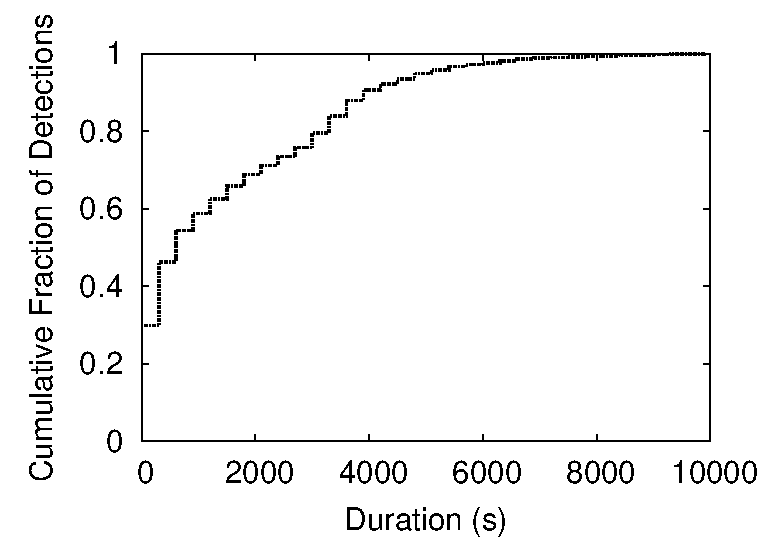
\includegraphics[width=1.05\columnwidth]{figs/patching/durationdetection/durationdetection.eps}
\caption{Distribution of the time it takes to remap all overlapping paths.}
\label{fig:overlap.delay.cdf}
%
\end{minipage}
\hfill
\begin{minipage}{0.32\textwidth}
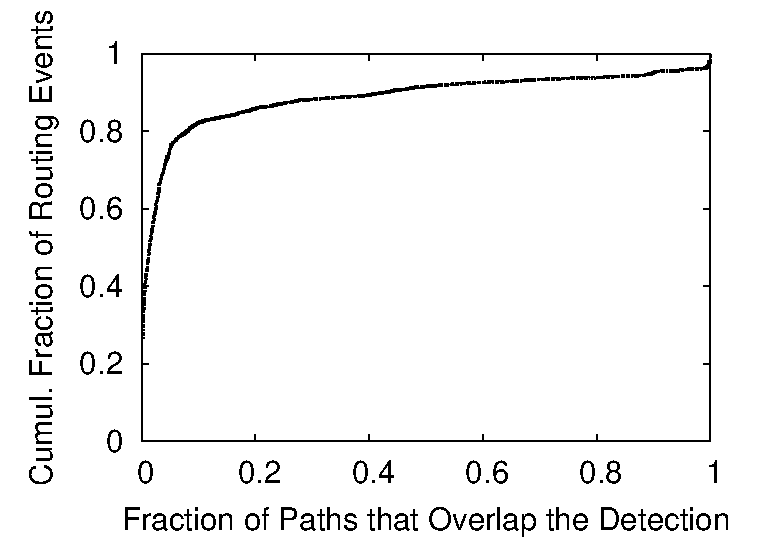
\includegraphics[width=1.05\columnwidth]{figs/patching/routesoverlapping/routesoverlapping.eps}
\caption{Fraction of monitored paths that overlap a routing event.}
\label{fig:overlap.quantity.cdf}
\end{minipage}
%
\hfill
\begin{minipage}{0.32\textwidth}
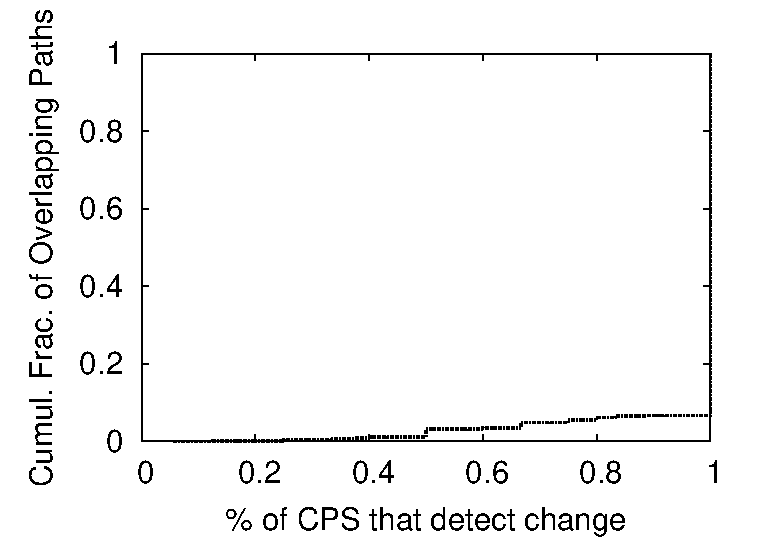
\includegraphics[width=1.05\columnwidth]{figs/patching/overlapcoverage/overlapcoverage_only_lczd.eps}
\caption{Prob.~of detecting change probing random radii in $\cps(q)$.}
\label{fig:lczd.intersection}
\end{minipage}
\end{figure*}

\section{Remapping Routing Events}
\label{sec:patching}

Routing events impact multiple paths in the Internet. Current
monitoring techniques monitor paths independently: detecting
a routing event on one Internet paths does not trigger any action on
other possibly-impacted paths.  This approach leads to outdated
routing information (as we do not remap other paths that have
changed due to the routing event) and prevents us from observing the
extent of a routing event (as another routing event might happen
before we remap all routes impacted by the first one).  We now
investigate whether we can use information about a just-remapped
change to efficiently (using few probes) detect and remap changes
the underlying routing event caused on other paths.

% Our goal is to
% develop techniques to efficiently (using few probes) identify and
% remap paths impacted by a routing event.

We define a \emph{local change zone domain}, denoted $\lczd(r')$,
for a change detected at radius $r'$ as the hops removed from the
previous path, $p_{i-1}$, around $r'$ plus the surrounding
divergence and convergence hops.  More formally, if $r_d$ and $r_c$
are the radii of the divergence and convergence hops, respectively,
and if $r^\prime_d = p_{i-1}\langle p_i[r_d]\rangle$ and $r^\prime_c
= p_{i-1}\langle p_i[r_c]\rangle$ are the radii of the divergence
and convergence hops on the previous path, then $\lczd(r')$ is
defined as the set of hops in $p_{i-1}$ between $r^\prime_d$ and
$r^\prime_c$, i.e., $\lczd(r') = \{p_{i-1}[x] \mid{} r^\prime_d \le
x \le r^\prime_c\}$.  A local change zone domain is similar to
a local change zone, but includes hops from the previous route
instead of hops from the new route.

\paragraphnd{Dataset.}  Upon detecting a path change at radius $r'$
on path $p_{i-1}$ (i.e., $p_i[r'] \ne p_{i-1}[r']$), \dtrack{}
immediately queues path $p_{i-1}$ to be remapped (remapping starts
immediately if there are no ongoing remaps).  We extended \dtrack{}
to collect data to study techniques for remapping paths after
detection of a \emph{routing event}.  After remapping of path
$p_{i-1}$ is complete, our extended \dtrack{} computes $\lczd(r')$
and proceeds to immediately remap all other paths that could be
impacted by the routing event.  More precisely, \dtrack{} enqueues
all (other) \emph{overlapping paths} $q$ which intersect
$\lczd(r')$, i.e., $q\, \cap\,\lczd(r') \ne \emptyset$, for
remapping (if not already queued).  Although this approach does not
guarantee \dtrack{} remaps all paths impacted by the routing event,
it still provides a more accurate snapshot of a routing event.  If
\dtrack{} detects a change in an overlapping path (remapped due to
a previously-detected routing event), \dtrack{} does not consider
the change a new routing event and does not enqueue paths for
remapping.  To prevent flapping routes and measurement noise from
enqueueing a constant stream of remappings, \dtrack{} limits the
number of remapped routing events per monitored path to four over
the last 24~hours.

We deployed the extended \dtrack{} on 80 PlanetLab nodes using three
sources of destinations: Alexa's TOP100 Websites,  RIPE Atlas
probes, and random reachable /24 prefixes. The total number of
destinations is 12763, which cover 5715 ASes using IP-to-AS mapping
information from iPlane. For each PlanetLab node, we selected 1000
random IP addresses to be monitored, allowing overlap among these IP
addresses across nodes. The data used in this analysis was collected
between Jan.~27th and Mar.~7th, 2016 (40 days).

% Let us denote the routing event by $E(p_{i-1})$ and let
% $D(E(p_{i-1}))$ be the time spent to remap all overlapping routes.

Figure~\ref{fig:overlap.delay.cdf} shows the CDF, over all remapped
routing events, of the time it takes to remap each event's
overlapping routes.  We round values to the nearest 5-minute
boundary.  Because we remap overlapping paths within a short period
(usually within one hour), there is a lower probability that
subsequent routing events will happen while the remap is ongoing.
Figure~\ref{fig:overlap.quantity.cdf} shows the CDF, over all
detected routing events, of the fraction of the 1000 monitored paths
that overlap with $\lczd(r')$.  We observe that 74\% of routing
events have at least one overlapping path, that most routing events
have a small (but significant) fraction of overlapping paths, and
that a few events (close to the monitoring node) impact all
monitored paths.

\paragraphnd{Efficient change detection.}  We now want to find a way
to identify whether an overlapping path has changed or remained
stable using few probes.  To this end, we consider sending probes to
overlapping paths at specific radii and checking for a change.  Let
$O(\lczd(r'), q)$ denote the overlap between the local change zone
domain $\lczd(r')$ for a routing event and an overlapping path $q$,
i.e., $\lczd(r')\cap{}q$.  We start with a \emph{candidate probing
set} $\cps(q)$ containing all radii between the first (closest to
the source) and last (furthest from the source) hops in
$O(\lczd(r'), q)$.

We find that probing the divergence hop $p_{i-1}[r^\prime_d]$ on the
overlapping path (i.e., probing radii $q\langle p_{i-1}[r^\prime_d]
\rangle$) rarely detects a path change.  As a result, we do not
consider probing the divergence hop to detect a change and remove
its radii from $\cps(q)$.\footnotemark{}  We also find that probing
the convergence hop on the overlapping path also rarely detects
a change, \emph{except} for routing events that change the
convergence's hop radii by adding or removing hops to the route.  As
a result, we only consider probing the convergence hop for routing
events that change the route length and remove its radii from
$\cps(q)$ otherwise.

\footnotetext{The divergence hop $p_{i-1}[r^\prime_d]$ may not be in
$O(\lczd(r'), q)$.  This happens whenever $q$ does not traverse
$p_{i-1}[r^\prime_d]$.  In this case, $\cps(q)$ is unchanged.}

% rarely no branch = 0.4%
% rarely no join onde nao muda o length = XXX%

Among the subset of overlapping paths that have changed, we find
that probing $\cps(q)$ can detect 86\% of changes.  Moreover, we
find that probing almost any radii in $\cps(q)$ will detect the
change.  \figstr~\ref{fig:lczd.intersection} shows the distribution
of the fraction of radii in $\cps(q)$ that can detect a change.  The
distribution shows that, for 97\% of the overlapping paths that
changed, probing any radii in $\cps(q)$ will detect a change.

\paragraphnd{Finding paths that change.}  We find that only 66\%
overlapping paths change.  Although the results above look
promising, they only apply to the 34\% of overlapping paths that
change.  We now look at mechanisms to efficiently identify which
paths have changed and which have not.
\figstr~\ref{fig:overlap.change.prob} shows, over all routing
events, the fraction of overlapping paths that changed.  We group
overlapping paths on the $x$ axis by the size of the overlap $O$
relative to $\lczd(r')$, i.e., $|O|/|\lczd|$.  We note that as
overlapping paths have bigger overlaps (i.e., have more in common
with the change), the higher the probability that the overlapping
path will change.  (This is more preliminary, but gives an idea
where we are headed right now.)

% cps cannot detect 4,83\% of changes

\begin{figure}
\begin{center}
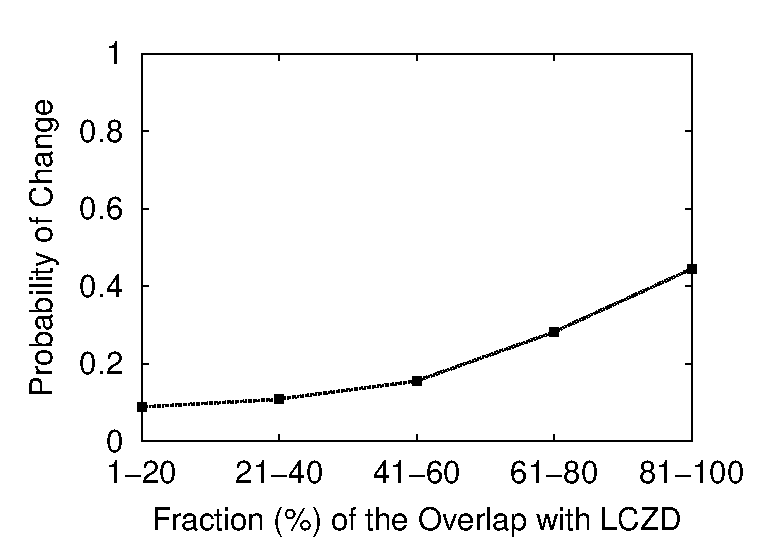
\includegraphics[width=1.05\columnwidth]{figs/patching/probchange/probchange.eps}
\caption{Probability of change as a function of overlap size.}
\label{fig:overlap.change.prob}
\end{center}
\end{figure}

% As described in Section~\ref{sec:char}, a path can have more than
% one change. This means that if $E(p_{i-1})$, has more than one
% $\lczd$, the \emph{overlapping paths} can cross different parts of
% $E(p_{i-1})$,.  Thus, we can divide $E(p_{i-1})$, in a more
% fine-grained parts ($\lczd$) which can explain better the
% behaviour of changes in \emph{overlapping paths}. For the rest of
% this section, we consider each $\lczd$ in $E(p_{i-1})$
% independently. 

% As pointed out before, a path change can have more than one
% $\lczd$ and we treat each of them independently in $E_p$.  We now
% formalize how we consider this fact inside \emph{overlapping
% paths}.

%We also looked
%at where the intersection $I$ is located compared to $\lczd$.  We
%find that XX\% of the intersections $I$ are at the start of the
%local change zone (i.e., $r_d + 1$), YY\% of the intersections $I$
%are at the end of the local change zone (i.e., $r_c - 1$), and that
%only ZZ\% of the intersections do are in neither extreme of the
%change zone.

% Let $\lczd'$ denote the local change zone domain of an
% \emph{overlapping path} without $r_d$ and $r_c$ if $|\lczd'_{p}|
% = |\lczd'_{p-1}|$, i.e., $\lczd'$ is the set of hops that reveal
% changes if probed. We define the overlapping change set $OCS
% = \bigcup(\lczd')$ as the set of all hops in the \emph{overlapping
% path} where a probe can detect a change.  


% vim: tw=68
